\section{Основная часть}

\begin{frame}
    \frametitle{Алгоритм}
    \begin{enumerate}
        \item Вычисление плотностей при помощи уравнений состояния.
        \item Нахождение давления и газонасыщенности методом
            Ньютона-Рафсона из условия равенства давления газа
            и жидкости.
        \item Вычисление скоростей законом Дарси.
        \item Переход на следующий шаг по времени согласно
            численной схеме.
    \end{enumerate}

\end{frame}

\begin{frame}
    \frametitle{Результаты}
     \begin{figure}[H]
         \centering
         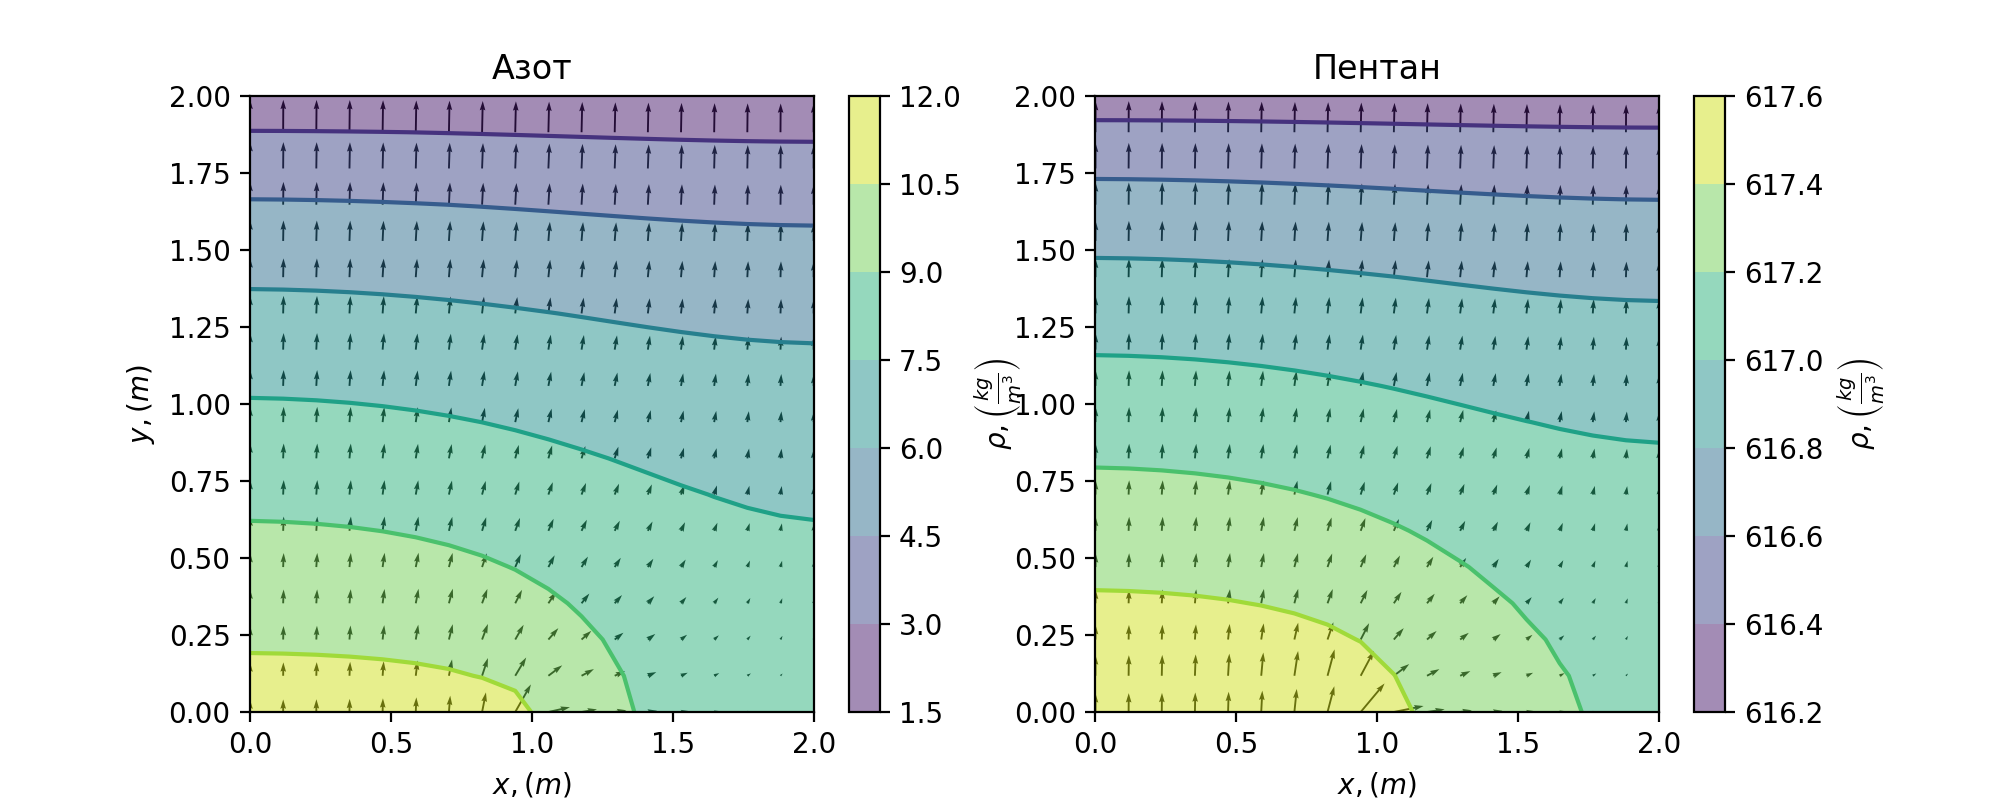
\includegraphics[width=\textwidth]
         {img/2phase-filtration-density.png}
     \end{figure}
\end{frame}

\begin{frame}
    \frametitle{Результаты}
     \begin{figure}[H]
         \centering
         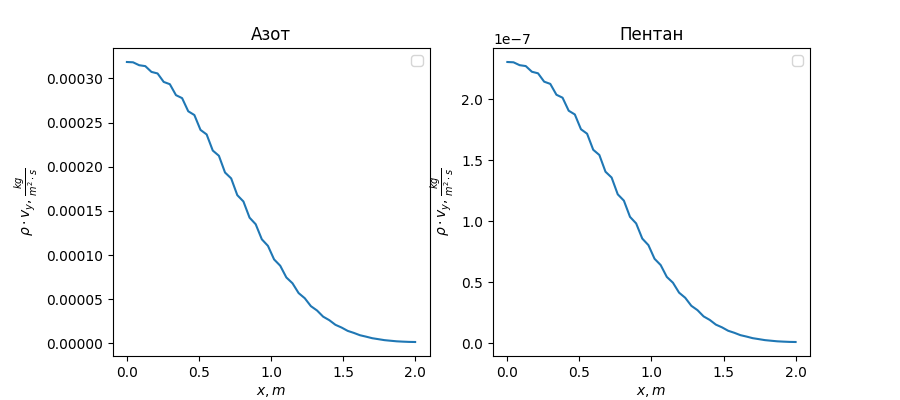
\includegraphics[width=0.9\textwidth]
         {img/flux.png}
     \end{figure}
\end{frame}
